\documentclass{article}
\usepackage[english]{babel}
\usepackage{spconf,amsmath,graphicx}
\usepackage{enumitem}
\setlist{nosep, leftmargin=14pt}
\usepackage{spconf,amsmath,graphicx,epsfig,multirow,subfigure}
\usepackage{hhline}                     % for merging cells in the table
\usepackage{array,ragged2e}     		% for aligning cells in tables
\usepackage{flushend}                   % for balancing the references
\usepackage{url}
\usepackage{dblfloatfix}
% Example definitions.
% --------------------

\usepackage{mwe} % to get dummy images

% Example definitions.
% --------------------
\def\x{{\mathbf x}}
\def\L{{\cal L}}



\newcolumntype{M}[1]{>{\centering\arraybackslash}m{#1}} % for centering all columns and rows
\newcolumntype{P}[1]{>{\centering\arraybackslash}p{#1}} % for centering all columns and rows
\newcolumntype{R}[1]{>{\raggedleft\arraybackslash}p{#1}} % for right-alignment all columns and rows
\newcolumntype{L}[1]{>{\raggedright\arraybackslash}p{#1}} % for left-alignment all columns and rows

% Commands for refer figs, eqs, and others
\newcommand{\figref}[1]{Fig.~\ref{fig:#1}}
\newcommand{\tblref}[1]{Table~\ref{tbl:#1}}
\newcommand{\eref}[1]{Eq.~\eqref{eq:#1}}
\newcommand{\secref}[1]{Section~\ref{sec:#1}}
\newcommand{\subsecref}[1]{Section~\ref{subsec:#1}}


\title{Design a neural network to generate a survival classifier for the Titanic dataset}

\name{Nguyen H. Hoang, Pham X. Cuong}
\address{Le Quy Don Technical University, Vietnam}

\begin{document}
\maketitle
\begin{abstract}
    The sinking of the Titanic is one of the most infamous shipwrecks in history.
    On April 15, 1912, during her maiden voyage, the widely considered “unsinkable” RMS Titanic sank after colliding with an iceberg.
    Unfortunately, there weren’t enough lifeboats for everyone onboard, resulting in the death of 1502 out of 2224 passengers and crew.
    In this report, we present a predictive model that answers the question: “what sorts of people were more likely to survive?” using passenger data (ie name, age, gender, socio-economic class, etc).
\end{abstract}


%-------------------------------------------------------------------------------------
% Introduction
%-------------------------------------------------------------------------------------
\section{Introduction}
\label{sec:intro}
In this report, we have gain access to two similar datasets that include passenger information like name, age, gender, socio-economic class, etc. One dataset is titled `train.csv` and the other is titled `test.csv`.
Train.csv will contain the details of a subset of the passengers on board (891 to be exact) and importantly, will reveal whether they survived or not, also known as the “ground truth”.
The `test.csv` dataset contains similar information but does not disclose the “ground truth” for each passenger. It’s your job to predict these outcomes.
Using a neural network for traning in the train.csv data, predict whether the other 418 passengers on board (found in test.csv) survived.
\begin{itemize}
    \item The dataset have \textbf{11} features: \textit{PassengerId}, \textit{Pclass}, \textit{Name}, \textit{Sex}, \textit{Age}, \textit{SibSp}, \textit{Parch}, \textit{Ticket}, \textit{Fare}, \textit{Cabin}, \textit{Embarked} and \textit{Survived}.
    The \textit{Survived} show that \textbf{2} labels Survived or not with \textbf{1} and \textbf{0}.
    \item While there was some element of luck involved in surviving,
    it seems some groups of people were more likely to survive than others.
    So we will figure out that with neural network.
    \item By using a Multilayer perceptron (MLP) neural network, we can predict the outcome of the survival of the passengers.
    \item In this report, we will show how to use the `train.csv` dataset to train a neural network and then use the trained model to predict the outcome of the survival of the passengers in the `test.csv` dataset. 
\end{itemize}

%-------------------------------------------------------------------------------------
% Proposed method
%-------------------------------------------------------------------------------------
\section{Method}

\begin{itemize}
    \item Preprocessing the data:
        \begin{itemize}
            \item In the dataset, we drop \textit{PassengerId}, \textit{Name}, and \textit{Ticket},
            Because they are unique by each passenger.
            We also drop \textit{Cabin} because total of dataset have \textbf{891} samples and \textit{Cabin} have \textbf{687} is \textbf{None}.
            \begin{center}
                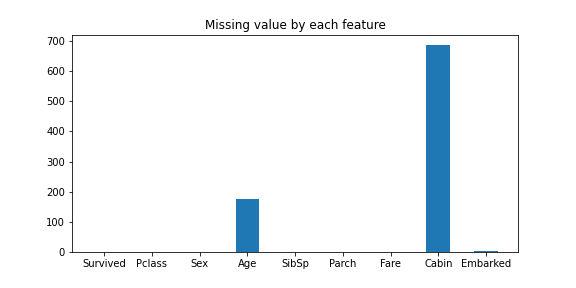
\includegraphics[width=0.425\textwidth]{missing.png}   
            \end{center}
            \item Normalize the data, we vectorize from discrete value to unique number value and use MinMaxScaler to normalize data.
            \[
               X_{new} = \frac{X - X_{min}}{X_{max} - X_{min}}
            \]
            \item Impute the missing values in \textit{Age} and \textit{Embarked},
            we use KNN algorithm to impute the missing values with \textbf{N neighbors} is 2 and formula caculate distance is \textbf{nan euclidean distances} .
            \[
            NED(x,y) = \sqrt{\frac{S}{S_{nnan}} \sum^n_{i=0} d(x,y)^2 }  
            \]
            \item Split the data into training, testing sets and validation sets with ratio is \textbf{7}:\textbf{2}:\textbf{1}.
        \end{itemize}
    \item Build a Multilayer perceptron (MLP) neural network with the following hyperparameters:
        \begin{itemize}
            \item \textbf{Number of input layers} is \textbf{7} from the input shape of the dataset after processed.
            \item \textbf{Number of hidden layers} is \textbf{3} and \textbf{number of neurons} in each layer is \textbf{8}.
            \item \textbf{Number of output layers} is \textbf{1} for classification is survival or not.
        \end{itemize}
    \begin{center}
        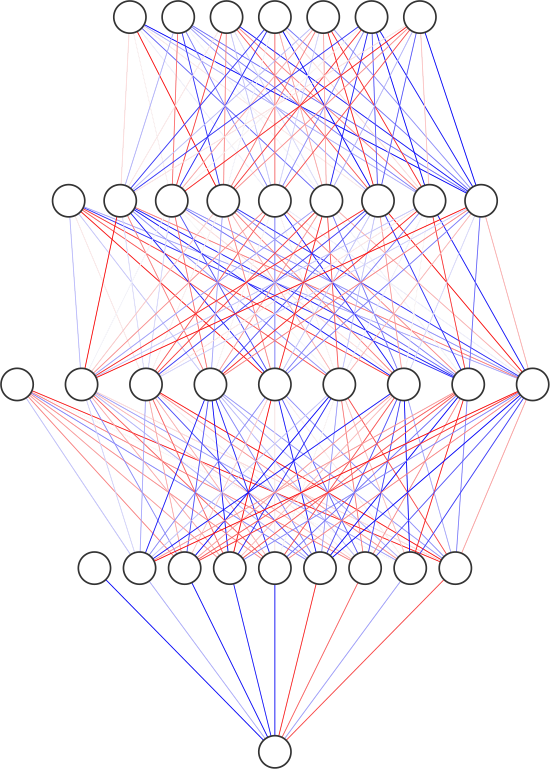
\includegraphics[width=0.425\textwidth,height=10cm]{nn.png}   
    \end{center}
    % \item Method,
    % \item Method,
    % \item Method,
    \item Method,
\end{itemize}
%-------------------------------------------------------------------------------------
% Experimental results and analysis
%-------------------------------------------------------------------------------------
\section{Experimental results and analysis}
\label{sec:results_analysis}
This section shows:
\begin{itemize}
    \item Dataset(s),
    \item Experimental setup,
    \item Evaluation methods,
    \item Experimental results,
    \item Analysis/discussion of the results.
\end{itemize}

%-------------------------------------------------------------------------------------
% Discussions
%-------------------------------------------------------------------------------------
\section{Conclusion}
\label{sec:conclu}
This section concludes what has been done in this report. The advantages, disadvantage, and the future direction also are shown in this section.

%-------------------------------------------------------------------------------------
% References
%-------------------------------------------------------------------------------------
% \section{REFERENCES}
% 
% References should be produced using the bibtex program from suitable
% BiBTeX files (here: strings, refs, manuals). The IEEEbib.bst bibliography
% style file from IEEE produces unsorted bibliography list.
% -------------------------------------------------------------------------
\bibliographystyle{IEEEbib}
\label{sec:refs}
\bibliography{refs}

\end{document}
